\documentclass[addpoints,12pt,ngerman]{exam}
\usepackage[utf8]{inputenc}
\usepackage[T1]{fontenc}
\usepackage{booktabs}
\usepackage{babel}
\usepackage{graphicx}
\usepackage{csquotes}
\usepackage{paralist,tikz,pgfplots}
\usepackage{xcolor,siunitx}


\pointpoints{Punkt}{Punkte}
\bonuspointpoints{Bonuspunkt}{Bonuspunkte}
\renewcommand{\solutiontitle}{\noindent\textbf{Lösung:}\enspace}
 
\chqword{Frage}   
\chpgword{Seite} 
\chpword{Punkte}   
\chbpword{Bonus Punkte} 
\chsword{Erreicht}   
\chtword{Gesamt}

\newcommand{\dozent}{Dr. Uwe Ziegenhagen}
\newcommand{\fach}{Klausur Statistik}
 
\pagestyle{headandfoot}
\runningheadrule \firstpageheadrule
\firstpageheader{}{}{\dozent \\ \fach}
\runningheader{}{}{\dozent \\ \fach}
\firstpagefooter{}{}{\thepage\,/\,\numpages}
\runningfooter{}{}{\thepage\,/\,\numpages}

\begin{document}

\begin{questions}
\question[5]  Zeichnen Sie die Funktion $3x^2+4x+5$!

\begin{solutionorgrid}[8cm]
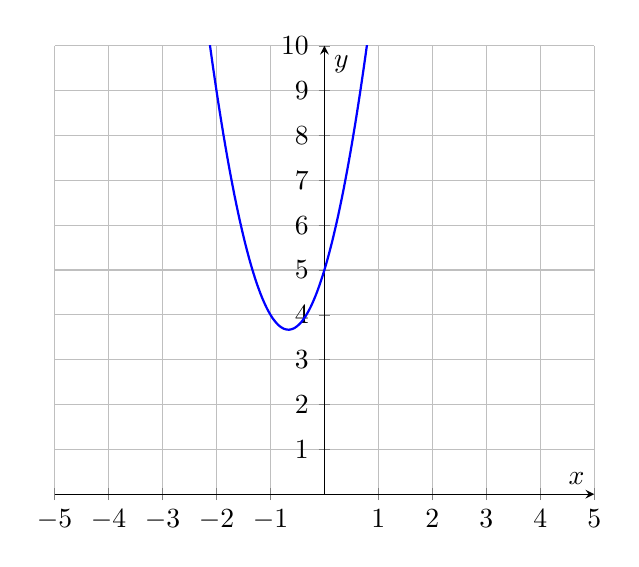
\begin{tikzpicture}[baseline]
\begin{axis}[
axis y line=center,
axis x line=middle,
grid=both,
xmax=5,xmin=-5,
ymin=0,ymax=10,
xlabel=$x$,ylabel=$y$,
xtick={-5,...,5},
ytick={0,...,11},
anchor=center,
]
\addplot[smooth,blue,thick,samples=100]{3*x^2+4*x+5} ;
\end{axis}
\end{tikzpicture}
\end{solutionorgrid}

\end{questions}
\end{document}